\documentclass[bibtotoc,liststotoc,BCOR=5mm,DIV=12]{scrbook}

% use this declaration to set specific page margins
%\usepackage[a4paper , lmargin = {2.7cm} , rmargin = {2.9cm} , tmargin = {2.7cm} , bmargin = {4.6cm} ]{geometry}
\usepackage[a4paper]{geometry}

\usepackage[ngerman, english]{babel}
\usepackage[backend=biber, style=numeric, sortcites=true]{biblatex}
\usepackage[T1]{fontenc} % german characters
\usepackage{graphicx} 				% it's recommended to use PDF images but you can use JPG or PNG as well
\usepackage{url}           		% format URLs
\usepackage{hyperref} 				% create hyperlinks
\usepackage{listings, color}	% for source code
\usepackage{subfig}						% two figures next to each other (example: figure 3a), figure 3b)
\usepackage{scrlayer-scrpage}					% header and footer line
\usepackage{todonotes}
\usepackage{blindtext}
\usepackage{hyperref}
\usepackage{float}
% header and footer line - no header & footer line on pages where a new chapter starts
% \pagestyle{scrheadings}
% \ohead{Design and Implementation of X}
% \ihead{Your Name}
% \ofoot[]{\thepage}
% \ifoot{Thesis, TU Berlin, DAMS, 2024} 

% set path where images are stored
\graphicspath{{./figures/}}

%
% der Befehl \hypenation versteht keine Sonderzeichen, also weder ä
% noch "a noch \"a. Wörter die derartige Zeichen enthalten müssen
% direkt im Text getrennt werden, z.B. Wör\-ter
%
\hyphenation{te-le-com-muni-cation 
te-le-com-muni-cation-specific 
Te-le-kom-mu-ni-ka-tions-API} 	
\addbibresource{./bib/references.bib} 				% use this file to set explicit hyphenations (doesn't seem to work correctly)

\usepackage{amsmath} % Ensure amsmath is included



\begin{document}
% ---------------------------------------------------------------
\frontmatter
    \thispagestyle{empty}
\begin{center}

\vspace*{1.4cm}
{\LARGE \textbf{Technische Universität Berlin}}

\vspace{0.5cm}

{\large Big Data Engineering (DAMS)\\[1mm]}

Fakultät IV\\
Ernst-Reuter-Platz 7\\
10587 Berlin\\
https://www.tu.berlin/dams\\

\vspace*{1cm}


\includegraphics[width=4cm]{tu_logo}

\vspace*{1.0cm}

{\LARGE \todo{[Choose yours: Bachelor or Master's]} Thesis}\\ %Bachelor or Master's

\vspace{1.0cm}
{\LARGE \textbf{Learned Quantization Schemes}}\\
\vspace*{0.3cm}
{\LARGE \textbf{for Data-centric ML Pipelines}}\\
\vspace*{1.0cm}
{\LARGE Anuun Chinbat}
\\
\vspace*{0.5cm}
Matriculation Number: 0463111\\
20.01.2025\\ % 	date of submission
\vspace*{1.0cm}

Supervised by\\
Prof. Dr. Matthias Boehm \\
% Add additional co-supervisors here
M.Sc. Sebastian Baunsgaard



\end{center}


    \thispagestyle{empty}
    \cleardoublepage
    
    
    \newpage

\thispagestyle{empty}

\begin{large}

\vspace*{6cm}

\noindent
Hereby I declare that I wrote this thesis myself with the help of no more than the mentioned literature and auxiliary means.
\vspace{2cm}

\noindent
Berlin, 01.01.2024\\ % 	date of submission

\vspace{3cm}

\hspace*{7cm}%
\dotfill\\
\hspace*{8.5cm}%
\textit{(Signature \todo{[your name]})}

\end{large}
 
    \thispagestyle{empty}
    \cleardoublepage
    
    
    \thispagestyle{empty}
\vspace*{1.0cm}

\begin{center}
    \textbf{Abstract} \label{abstract}
\end{center}

\vspace*{0.5cm}

Machine learning (ML) models are notoriously resource-intensive.
Given their widespread application across every-day edge devices,
the need to reduce their memory and computing requirements is becoming ever more pressing.

Despite the said resource-intensiveness of ML models, at the same time 
they offer the main ingredient for the remedy to the malady - redundancy - 
which can be exploited to reduce their memory usage.

While the redundancy exploitation of ML models is already a common 
technique that comes in different forms, starting from pruning and
ending with ..., quantization presents itself as an especially promising 
area especically in the sense of learned quantization - 
the process of making ML models learn their optimal quantization parameters
on their own.

Hence, the current work employs two techniques that bypass the main issue of learned quantization,
that is, the non-differentiability of rounding operations.
While the first technique involves custom loss functions that directly take into account
quantization goals, the second approach incorporates a custom gradient calculation that is
easily integratable to various training scenarios.

As a result of these two techniques, a memory usage reduction of up to ..x is obtained 
on MNIST, CIFAR10, and Imagenette. 

\begin{enumerate}
    \item The problem:
        \begin{enumerate}
            \item High memory usage
            \item Models are redundant
        \end{enumerate}

    \item Why it's an interesting problem
        \begin{enumerate}
            \item \{I need something about current techniques not being enough\}
            \item \{Also something about learned quantization specifically that's not enough\}
        \end{enumerate}
        Despite the said resource-intensiveness of ML models, they 

    \item What our solution achieves
        \begin{enumerate}
            \item Custom loss functions that encourage quantization
            \item Custom gradient calculation that encourages quantization only where it's necessary 
        \end{enumerate}            
    \item What follows from our solution
        \begin{enumerate}
            \item Reduced memory requirement of X with accuracy degradation within Y \%.
        \end{enumerate}   
\end{enumerate}

    \thispagestyle{empty}
    \cleardoublepage
    
    \thispagestyle{empty}
\vspace*{0.2cm}

\begin{center}
    \textbf{Zusammenfassung} \label{zusammenfassung}
\end{center}

\vspace*{0.2cm}

\noindent 
This is a placeholder for the german abstract (Kurzfassung) which should follow the same structure as the abstract.
    \thispagestyle{empty}
    
    
    \tableofcontents
    \thispagestyle{empty}
    
% --------------------------------------------------------------

\mainmatter % comment single chapters for faster compilation

    \chapter{Introduction\label{cha:chapter1}}

\hspace{1em}Such is the life of a modern human being that not a single day passes 
without a machine learning model toiling away in the background. 
From unlocking one's phone with Face ID in the morning 
to receiving a curated recommendation feed on Netflix in the evening - 
all is ML - but at what cost?

If we consider GPT-3 as an example, 
its 175 billion parameters need a whopping 700 gigabytes of storage in total - 
4 bytes for each parameter represented in single-precision floating-point format (FP32).
This costliness of modern ML models has revitalized interest in the research area
of \textit{quantization of Neural Networks} (NNs) 
which aims to reduce model size by developing methods 
that directly or indirectly decrease the amount of memory 
needed to store parameters numbering in the millions or billions. 
Going back to the GPT-3 example, by directly clamping its FP32 parameters 
to an 8-bit integer (INT8) representation, we can reduce its storage requirement 
from 700 to just 175 gigabytes. 

But what costs does quantization itself entail? The natural answer to this question 
would be a reduction in model performance, as a decrease in precision logically implies 
a decrease in accuracy. However, there is a somewhat counterintuitive phenomenon where 
quantization improves accuracy by introducing discretization effects, which act like a
form of regularization, forcing the model to generalize better. No matter whether quantization
results in better or a slightly worse performance, the conclusion is that 
for each model there is an optimal way to quantize it within reasonable degradation ranges.
And if the model is able to learn its optimal parameters, 
it is most likely also able to learn its optimal quantization parameters. 

The fact that, indeed, models can learn their optimal quantization parameters has been proven 
many times in the past. But is there a way to make them do it better - is a question 
that will always remain and to which this thesis aims to contribute. In that sense, 
the current work will explore non-standard ways to tackle the two main problems that the process 
of learning optimal quantization parameters poses. First, how to overcome the issue 
of non-differentiability of rounding operations in the back-propagation. Second, how
to encourage the model to quantize only where it's necessary and feasible. 


This paragraph is gonna be about how previous reseacrh has tried to tackle the wbove two questions.


Finally, factually, how this thesis implemented the actions to the goal.
    \chapter{Background\label{cha:chapter2}}

This chapter addresses the theoretical and contextual background 
necessary to understand the key concepts and methodologies 
that form the foundation of the current research.
The first section will discuss the basics of deep NNs, 
upon which the technical setup of this thesis is based.
The next section aims to provide a broader context for the term quantization, 
followed by a final section that explains common techniques of \textit{learned quantization}, 
as well as the trade-offs and challenges they present. 


% ------------------------------------------------------------
% ----------------------- deeplearning ----------------------- 
% ------------------------------------------------------------
\section{Fundamentals of Deep Learning}
\label{sec:deeplearning}
This section introduces the fundamental concepts of deep learning, 
beginning with the most basic NN architecture components \ref{subsec:denseconvolutional} and progressing to loss functions with regularization \ref{subsec:lossregularization}. 
The concepts of the forward pass and backpropagation will be explained in the last subsection \ref{subsec:forwardback}.

% -------------------- denseconvolutional --------------------
\subsection{Dense and Convolutional Layers}
\label{subsec:denseconvolutional}
NNs can be considered a mathematical abstraction of the human decision-making process. 
Consider a scenario where, given an image, you need to say aloud what you see. 
The two eyes can be regarded as input nodes that receive the initial data, 
the brain can be seen as a set of \textit{hidden layers} that process this data, 
and your mouth — the output node that provides the final answer.
\\
\\
A hidden layer, which typically consists of many neurons, is where the magic
 — or the transformation of data — happens. In its simplest form, 
 within the classic \textit{Multilayer Perceptron} (MLP) model,
 each hidden layer neuron performs a weighted operation:

\[
\textit{output} = f(w \cdot \textit{input} + b)
\]
\\
\noindent where:

\begin{itemize}
  \item \textit{input} refers to the outputs from the previous layer (or the initial data from input nodes) that are fed into a specific neuron in the hidden layer.
  \item \textit{w} (weights) is a vector of parameters associated with that specific neuron, defining the importance of each input received by this neuron. 
  \item \textit{b} (bias) is an additional scalar parameter specific to the neuron, which shifts the result of the weighted sum, allowing for more flexibility.
  \item \textit{f} is the \textit{activation function}, a nonlinear function applied to the weighted sum of inputs and bias in that specific neuron, allowing for more complexity.
  \item \textit{output} is the result produced by the neuron, which will then be passed on to the next hidden layer (or to the final output layer).
\end{itemize}

\noindent Hidden layers where each neuron is connected to every neuron in the previous layer 
and every neuron in the next layer are called \textit{dense layers}.

\begin{figure}[h!]
  \centering
  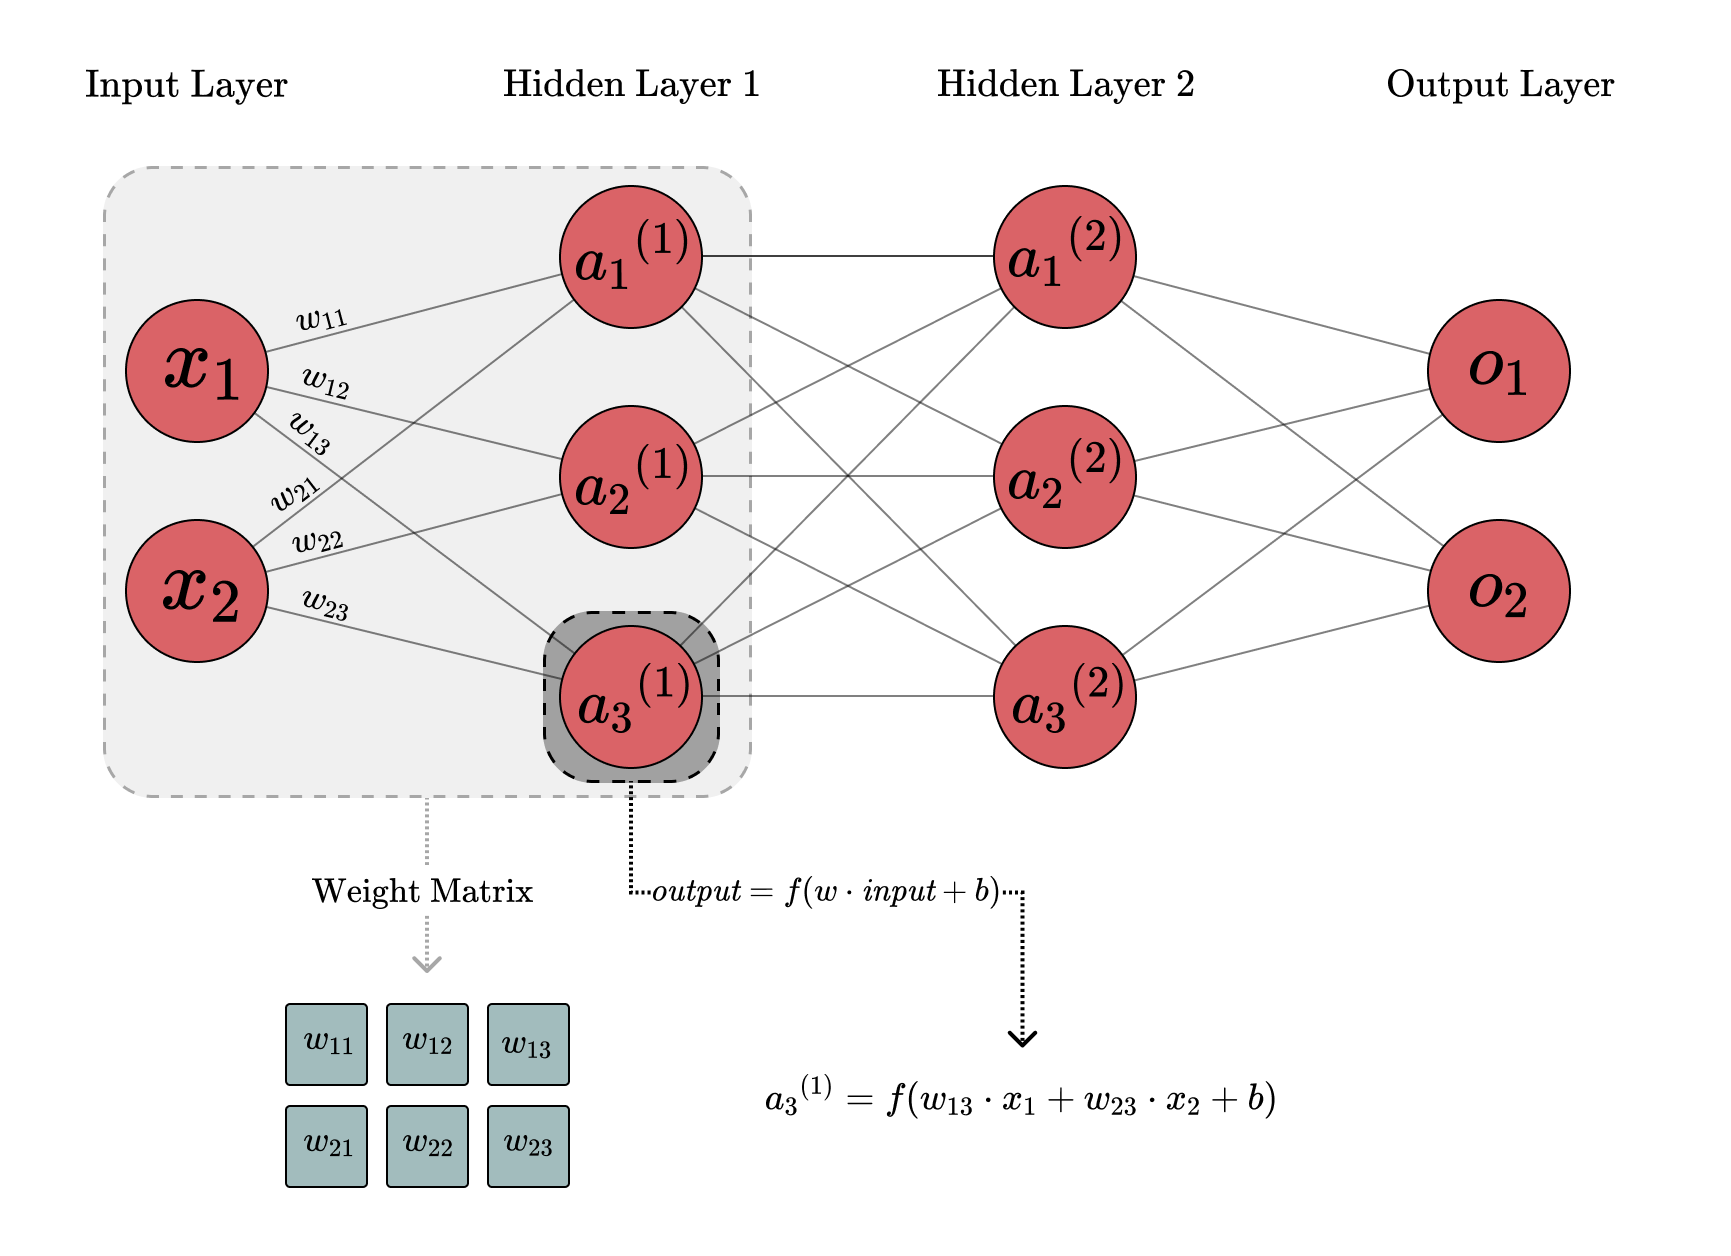
\includegraphics[width=14cm]{dense_layer}
  \caption{An example of a NN with two hidden dense layers, showing the connections between neurons in adjacent layers.}
  \label{fig:dense_layer}
\end{figure}

\noindent Mathematically, dense layers can be represented as:

\[
\textit{a} = f(W \cdot \textit{x} + b)
\]
\\
\noindent where:
\begin{itemize}
  \item \textit{x} is the input vector, representing outputs from the previous layer (or initial input data for the first layer).
  \item \textit{W} is the \textit{weight matrix}, with each row corresponding to the weight vector \( w \) of a specific neuron.
  \item \textit{b} represents the bias vector, where each scalar element corresponds to the bias of a specific neuron.
  \item \textit{f} is the \textit{activation function} that is applied element-wise.
  \item \textit{a} refers to the output vector, representing the activations of all neurons.
\end{itemize}

\noindent This interconnectedness of dense layers introduces the inherent redundancy, 
or the over-parameterizedness of NNs \cite{gholami2021survey}. It is particularly true in models with a large number of neurons, 
where \( W \) results in a vast number of parameters, which do not contribute to the model accuracy equally \cite{hubara2016qnn}.
\\
\\
\noindent \textit{Convolutional layers} are another type of hidden layers 
that involve a \textit{convolution} operation on the input. Intuitively, a standard convolution is 
a process of sliding a small grid over an input to find patterns. The figure below, for example, shows 
the application of the Sobel kernel that detects edges on the input image.

\begin{figure}[h!]
  \centering
  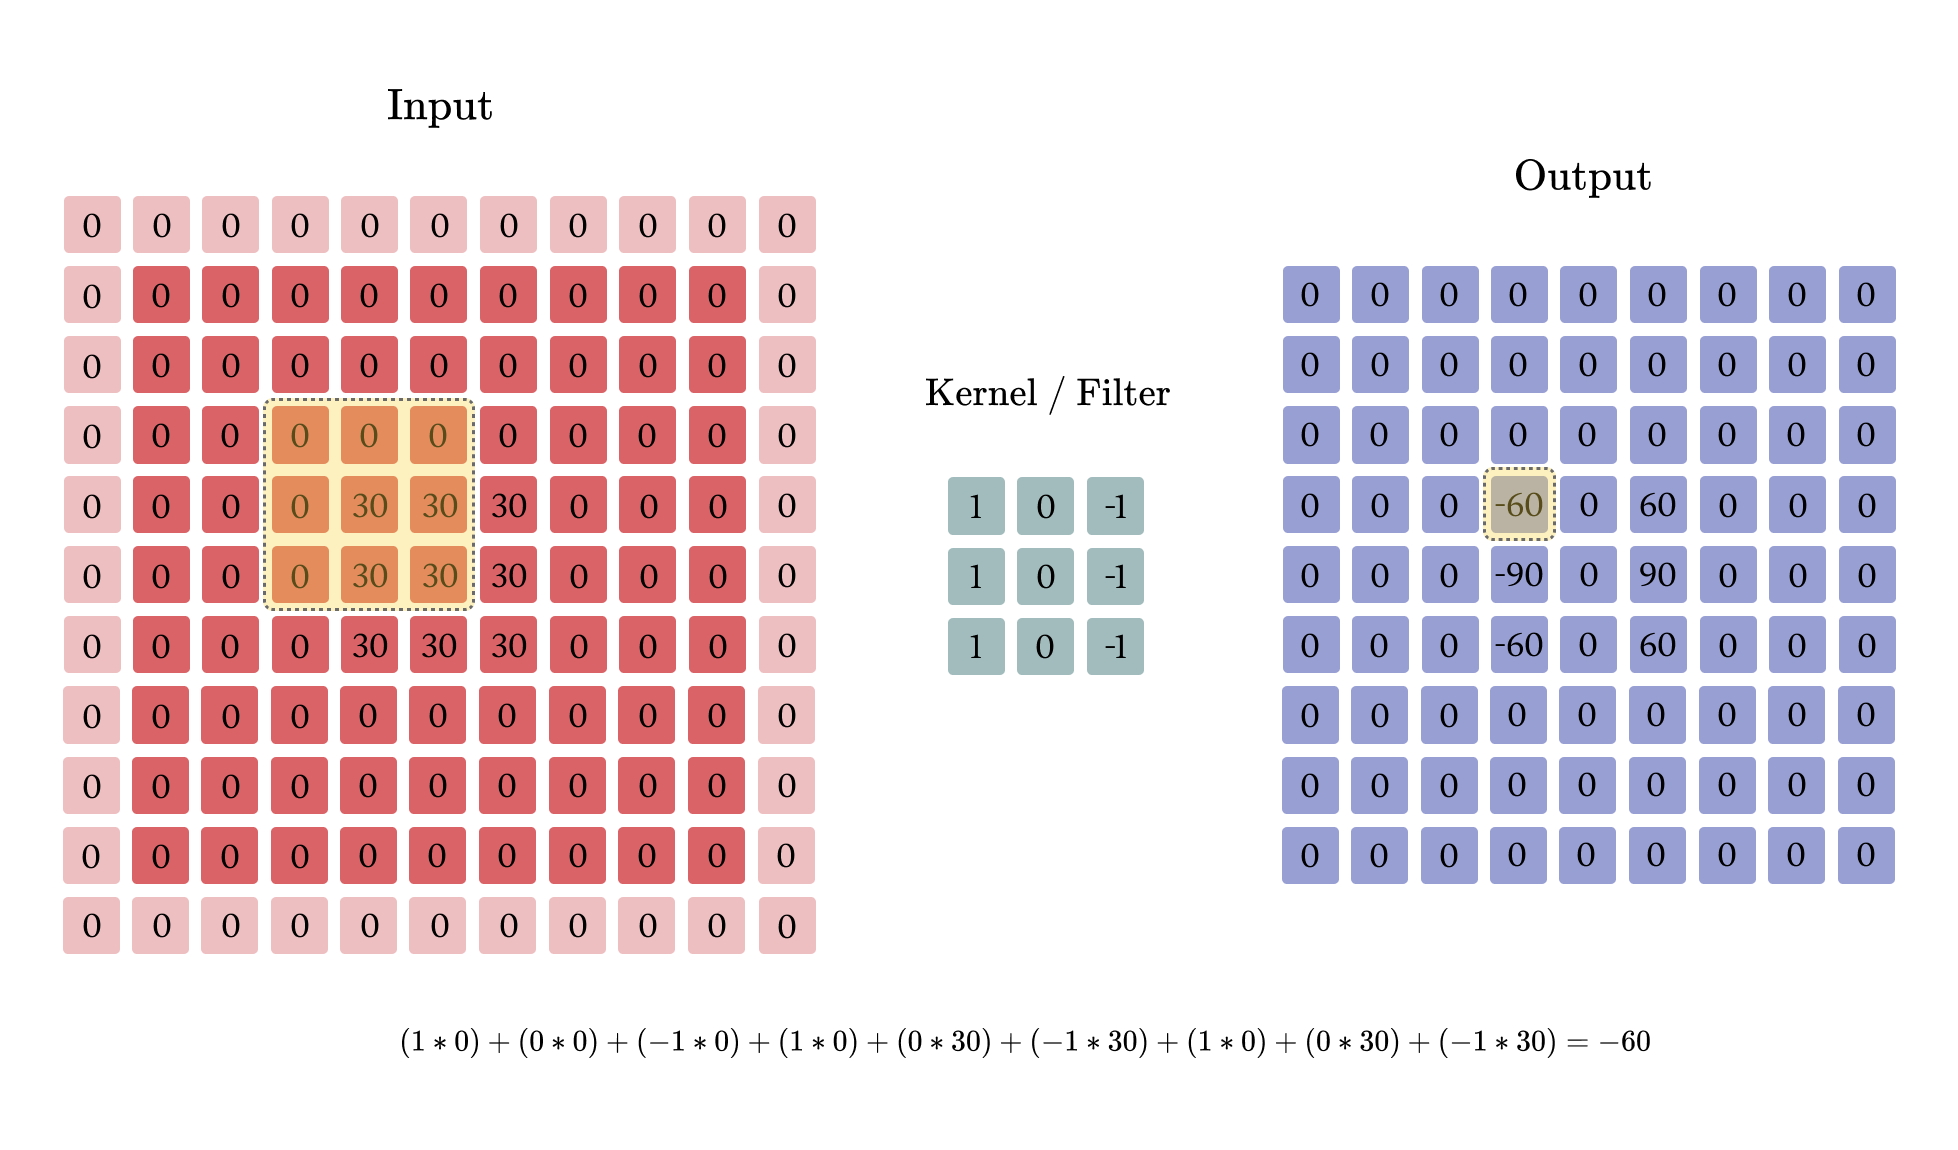
\includegraphics[width=14cm]{convolution}
  \caption{A 3×3 kernel (filter) sliding over a padded input matrix to compute the output feature map, demonstrating the interaction between the kernel weights and input values at a specific position.}
  \label{fig:convolution}
\end{figure}

\noindent For multi-channeled inputs, like RGB images, the convolution operation uses a multi-channeled kernel, as shown in Figure 2.3, 
producing a single-channeled feature map that combines weighted contributions from all input channels. 
A convolutional layer typically includes multiple such kernels, generating feature maps equal to the number of kernels.
After the convolution operation generates the feature maps, a bias term is added to each map, 
and the activation function is applied element-wise — just like in dense layers.

\begin{figure}[h!]
  \centering
  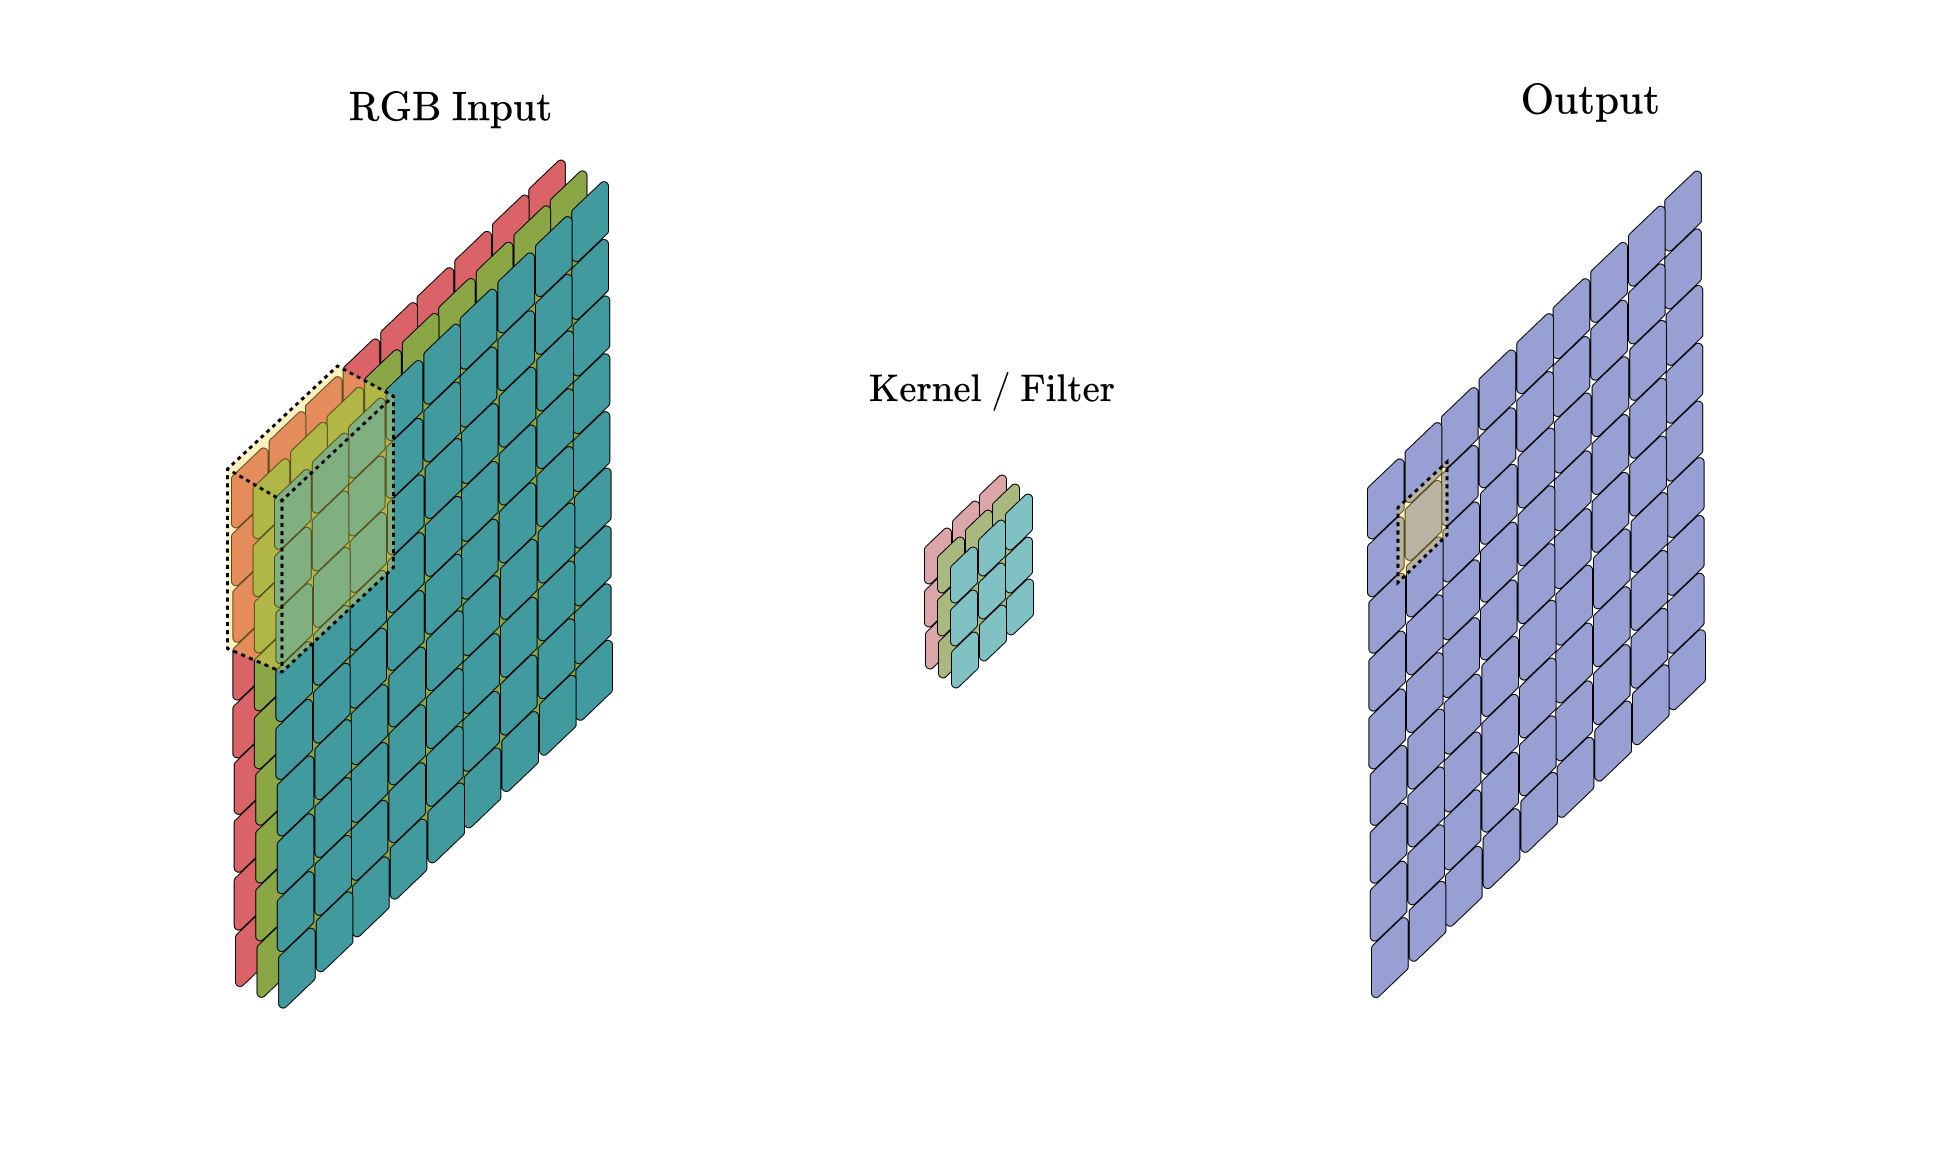
\includegraphics[width=14cm]{convolution_multiple_channels.png}
  \caption{A 3×3x3 kernel (filter) sliding over an RGB input matrix to produce a single-channeled output feature map.}
  \label{fig:convolution_multiple_channels}
\end{figure}

\noindent Mathematically, a convolutional layer can be represented as:

\[
y_{i,j,k} = \phi \left( \sum_{m=1}^M \sum_{p=1}^P \sum_{q=1}^Q x_{i+p-1, j+q-1, m} \cdot w_{p,q,m,k} + b_k \right)
\]
\\
\noindent where:
\begin{itemize}
  \item \( P, Q \) are the height and width of the filter, respectively.
  \item \( M \) is the number of input channels.
  \item \( y_{i,j,k} \) denotes the output at position \((i, j)\) for the \(k\)-th filter.
  \item \( x_{i+p-1, j+q-1, m} \) is the input at position \((i+p-1, j+q-1)\) for the \(m\)-th input channel.
  \item \( w_{p,q,m,k} \) represents the weight of the filter at position \((p, q)\) for the \(m\)-th input channel and \(k\)-th filter.
  \item \( b_k \) is the bias for the \(k\)-th filter.
  \item \( \phi(\cdot) \) is the activation function.
\end{itemize}

\noindent In simpler terms, a convolutional layer applies filter weights 
as it slides over rows \((p)\), columns \((q)\), and channels \((m)\), 
sums the results, adds bias \((b_k)\), 
and repeats this for all positions \((i, j)\) and filters \((k)\).
\\
\\
\noindent Although convolutional layers often have fewer weight parameters than dense layers in typical architectures, 
they still contain redundancies \cite{huang2017densely}, presenting an opportunity for quantization. 
Thus, both dense and convolutional layers will be the focus of this work.

% -------------------- lossregularization --------------------

\subsection{Loss Functions and Regularization}
\label{subsec:lossregularization}
The weights and biases are usually \textit{learnable parameters}
that the model adjusts during \textit{training}.
The training process of NNs is similar to how our brains learn from mistakes. 
Given the ground truth, a NN adjusts its learnable parameters 
using a specific function that compares the ground truth with the output generated by the network, 
essentially measuring the magnitude of the network's errors.
\\
\\
This function is called a \textit{loss function}, and depending on the type of question the network aims to answer, it can take many different forms.
For example, for the MLP described in Figure~\ref{fig:dense_layer} that generates a binary classification, we would use the \textit{log loss} function. 
Since the datasets used in this thesis involve multi-class classification, the \textit{sparse categorical cross-entropy} (SCCE) loss function will be used, 
which measures the difference between the predicted class probabilities and the true labels for each class in the dataset.
\\
\\
Often the loss function alone is not enough for a NN to perform well, 
as it may lead to overfitting or fail to capture desired generalization properties.
This is why a \textit{regularization term} that penalizes unwanted behaviours
is added to the loss function.
\\
\\
A typical regularization term is \( L_2 \), 
which penalizes large weights by adding the sum of the squared weights to the loss. 
The modified loss function is then expressed as:

\[
\mathcal{L}_{\text{total}} = \mathcal{L}_{\text{data}} + \lambda \sum_{i} w_i^2
\]
\\
\noindent where:

\begin{itemize}
  \item \( \mathcal{L}_{\text{data}} \) is the original loss function (in our case, the SCCE loss function).
  \item \( \lambda \) is a scalar parameter that controls the strength of the regularization.
  \item \( w_i \) represents each individual weight value in the model.
\end{itemize}

\noindent The current work employs multiple custom regularization terms 
that encourage specific behaviors in the models while discouraging others. 
These terms will be discussed in detail in the Experimental Setup section \ref{sec:setup}.

% -------------------- forwardback --------------------

\subsection{Forward-Pass and Back-Propagation}
\label{subsec:forwardback}
The repetition of the mathematical operations described earlier in the Dense and Convolutional Layers subsection \ref{subsec:denseconvolutional} 
during model training constitutes the \textit{forward pass}. 
It is the process where input data is passed through the network layer by layer, 
with each layer applying its learned weights and biases to produce a final output. 
\\
\\
As mentioned in the previous subsection, this output is then compared with the ground truth by the loss function that produces an error.
This error is used to update the learnable parameters in \textit{W} and \textit{b} during a process called \textit{back-propagation}.
\\
\\
In other words, back-propagation is the method by which the network adjusts its parameters to minimize the error. 
It calculates the gradient of the loss function with respect to each parameter using the chain rule. 
\( W \) and \( b \) are typically updated as follows:

\[
W = W - \eta \frac{\partial L}{\partial W}, \quad b = b - \eta \frac{\partial L}{\partial b}
\]
\\
\noindent where \( L \) is the loss function, and \( \eta \) is the learning rate.
\\
INSTEAD OF THIS WE NEED TO EXPLAIN HOW A CLASSICAL WEIGHT UPDATE LOOKS LIKE IN TENSORFLO
ALSO ADD how the theory looks like in tensorflow so that it's easier to follow
\\
For example, consider the weight \( W_{I1,H1_1} \) represented as the line between \textit{Input 1} and the hidden layer node \( H1_1 \) in Figure~\ref{fig:mlp_diagram}. 
The gradient of this weight with respect to the loss is calculated using the chain rule:

\[
\frac{\partial L}{\partial W_{I1,H1_1}} = \frac{\partial L}{\partial \text{Output 1}} \cdot \frac{\partial \text{Output 1}}{\partial H1_1} \cdot \frac{\partial H1_1}{\partial W_{I1,H1_1}}
\]

\noindent Where:
\begin{itemize}
    \item \( \frac{\partial L}{\partial \text{Output 1}} \) is the gradient of the loss with respect to \textit{Output 1}.
    \item \( \frac{\partial \text{Output 1}}{\partial H1_1} \) is the gradient of \textit{Output 1} with respect to the output of \( H1_1 \).
    \item \( \frac{\partial H1_1}{\partial W_{I1,H11}} \) is the value of \textit{Input 1}, since \( H1_1 \) is a weighted sum of the inputs.
\end{itemize}

\noindent This shows how each weight contributes to the final error during back-propagation.

% ----------------------- basics of quantization ----------------------- 

\section{Basics of Quantization}
\label{sec:section2}
This section aims to answer the \textit{why} question with respect to quantization and further provides a broader understanding of the term regarding its types.

\subsection{Purpose and Definition}
\label{subsec:subsection1}
With humans becoming increasingly dependent on deep learning models disguised as everyday tools on edge devices with 
limited capacities — the need for these models to function in a resource- and 
time-efficient manner is more imperative than ever. Among the many ways to meet this need, 
quantization has become one of the most popular techniques used to reduce the computational 
and memory costs of deep NNs.
\\
\\
The popularity of quantization stems from the inherent over-parameterization of NNs \cite{gholami2021survey},
which makes them generally \textit{robust} to precision reduction without significant degradation in performance \cite{DBLP:journals/tcad/DuLCPTW15}.
This robustness is akin to how near-sightedness does not prevent people from walking straight,
or how someone can still understand a text message filled with typos as long as the essential words are there.
\\
\\
Setting aside other possible real-life analogies, the term "quantization"— rooted in the early 20th century \cite{gray1998quantization} — 
formally refers to the process of reducing the bit precision of parameters while ensuring accuracy remains within an acceptable range.

\subsection{Common Quantization Approaches}
\label{subsec:subsection2}

There is a multitude of ways to classify NN quantization methods, a broader overview of which will be covered
in the Related Work chapter \ref{cha:chapter5}.
For now, we will focus on a few selected approaches from the general categories of both 
\textit{data-driven} and \textit{data-free} methods \cite{Edouard2022SPIQ} to provide a basic understanding of the NN quantization process.
\\
\\
The simplest form of data-free quantization, or \textit{post-training quantization} \cite{jiang2021efficient},
involves converting already trained parameters from FP32 to a lower bit-width format
without using the initial training data. 
A common approach is to apply \textit{uniform quantization} that maps real values to a set number
of \textit{bins}. The general formula can be written as:

\[
Q(r) = round(\frac{r}{S})
\]

\noindent Where:
\begin{itemize}
    \item $Q(\cdot)$ denotes the quantization operation.
    \item $r$ is the real value of a given model parameter in higher bit-width representation.
    \item $round(\cdot)$ is some rounding operation, such as a simple $floor(\cdot)$.
    \item $S$ is a scaling factor.
\end{itemize}

\noindent  As a result, we essentially end up with a discrete number of values in lower bit precision, 
instead of an almost continuous range of real numbers as shown in Figure \ref{fig:quantizing_example}.
\\
\begin{figure}[h!]
  \centering
  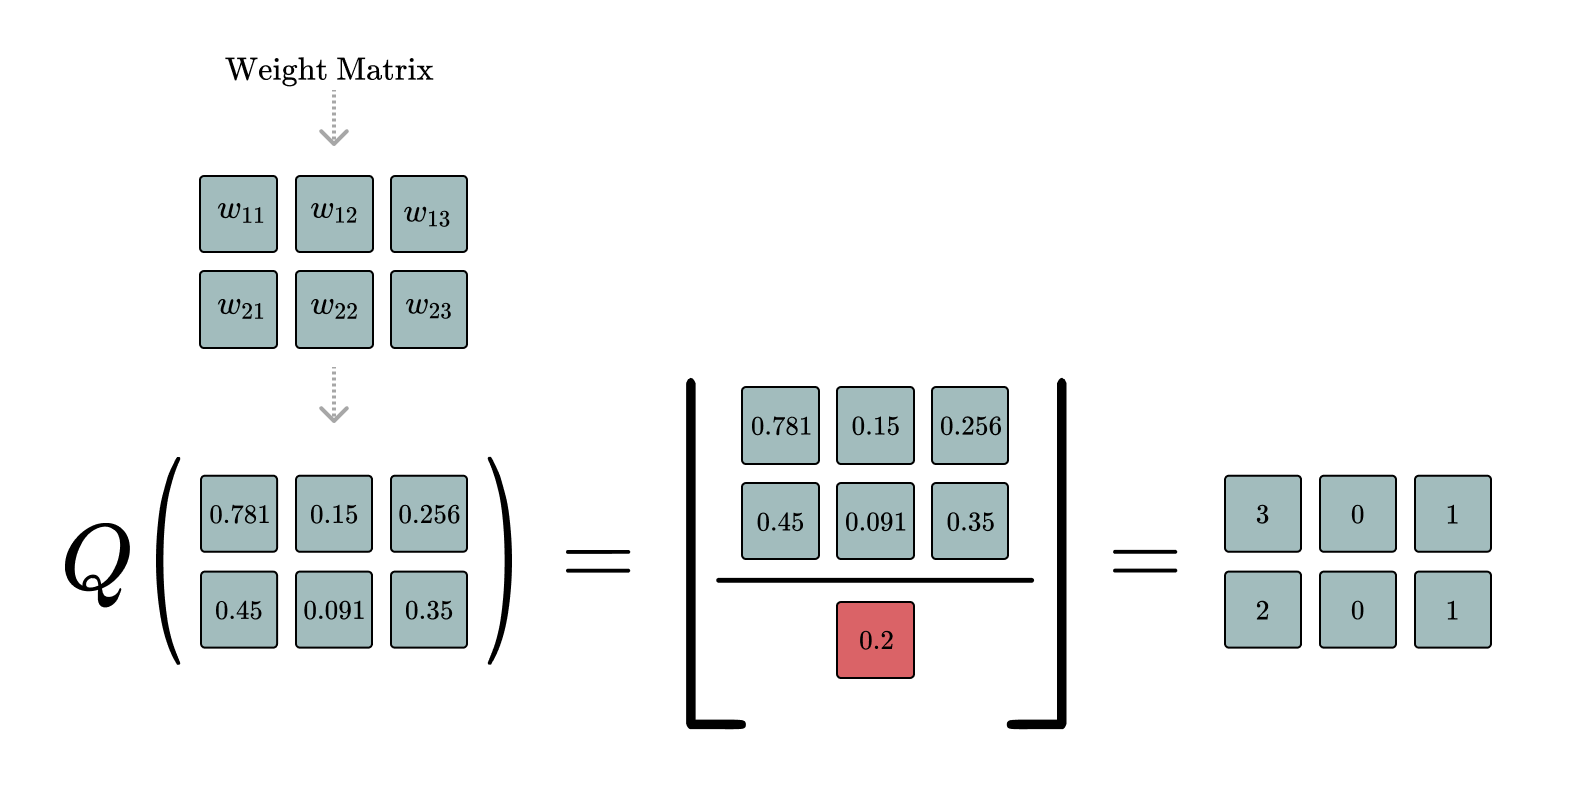
\includegraphics[width=10cm]{quantizing_example.png}
  \caption{An example illustrating the quantization operation on the weight matrix from Figure \ref{fig:dense_layer}, 
  with arbitrary values for demonstration purposes.}
  \label{fig:quantizing_example}
\end{figure}

\noindent Unlike data-free quantization  —  as the name suggests — data-driven quantization typically involves retraining the model
using the initial data. An example of this approach is the Ristretto framework \cite{DBLP:journals/tnn/GyselPMG18}, which, similar to data-free methods, 
first analyzes the trained model to select suitable lower bit-width number formats for its weights.
Then, using a portion of the original dataset, the framework determines appropriate formats for layer inputs and outputs.
As a next step, based on the validation data, Ristretto adjusts the quantization settings to achieve optimal performance 
under the given constraints. Finally, the quantized model is fine-tuned using the training data.
\\
\\
A much simpler example could be the min-max quantization on input data as shown in Figure \ref{fig:min_max_quantization}. 
This method is used by Tensorflow Lite as part of its post-training quantization process.

\begin{figure}[h!]
  \centering
  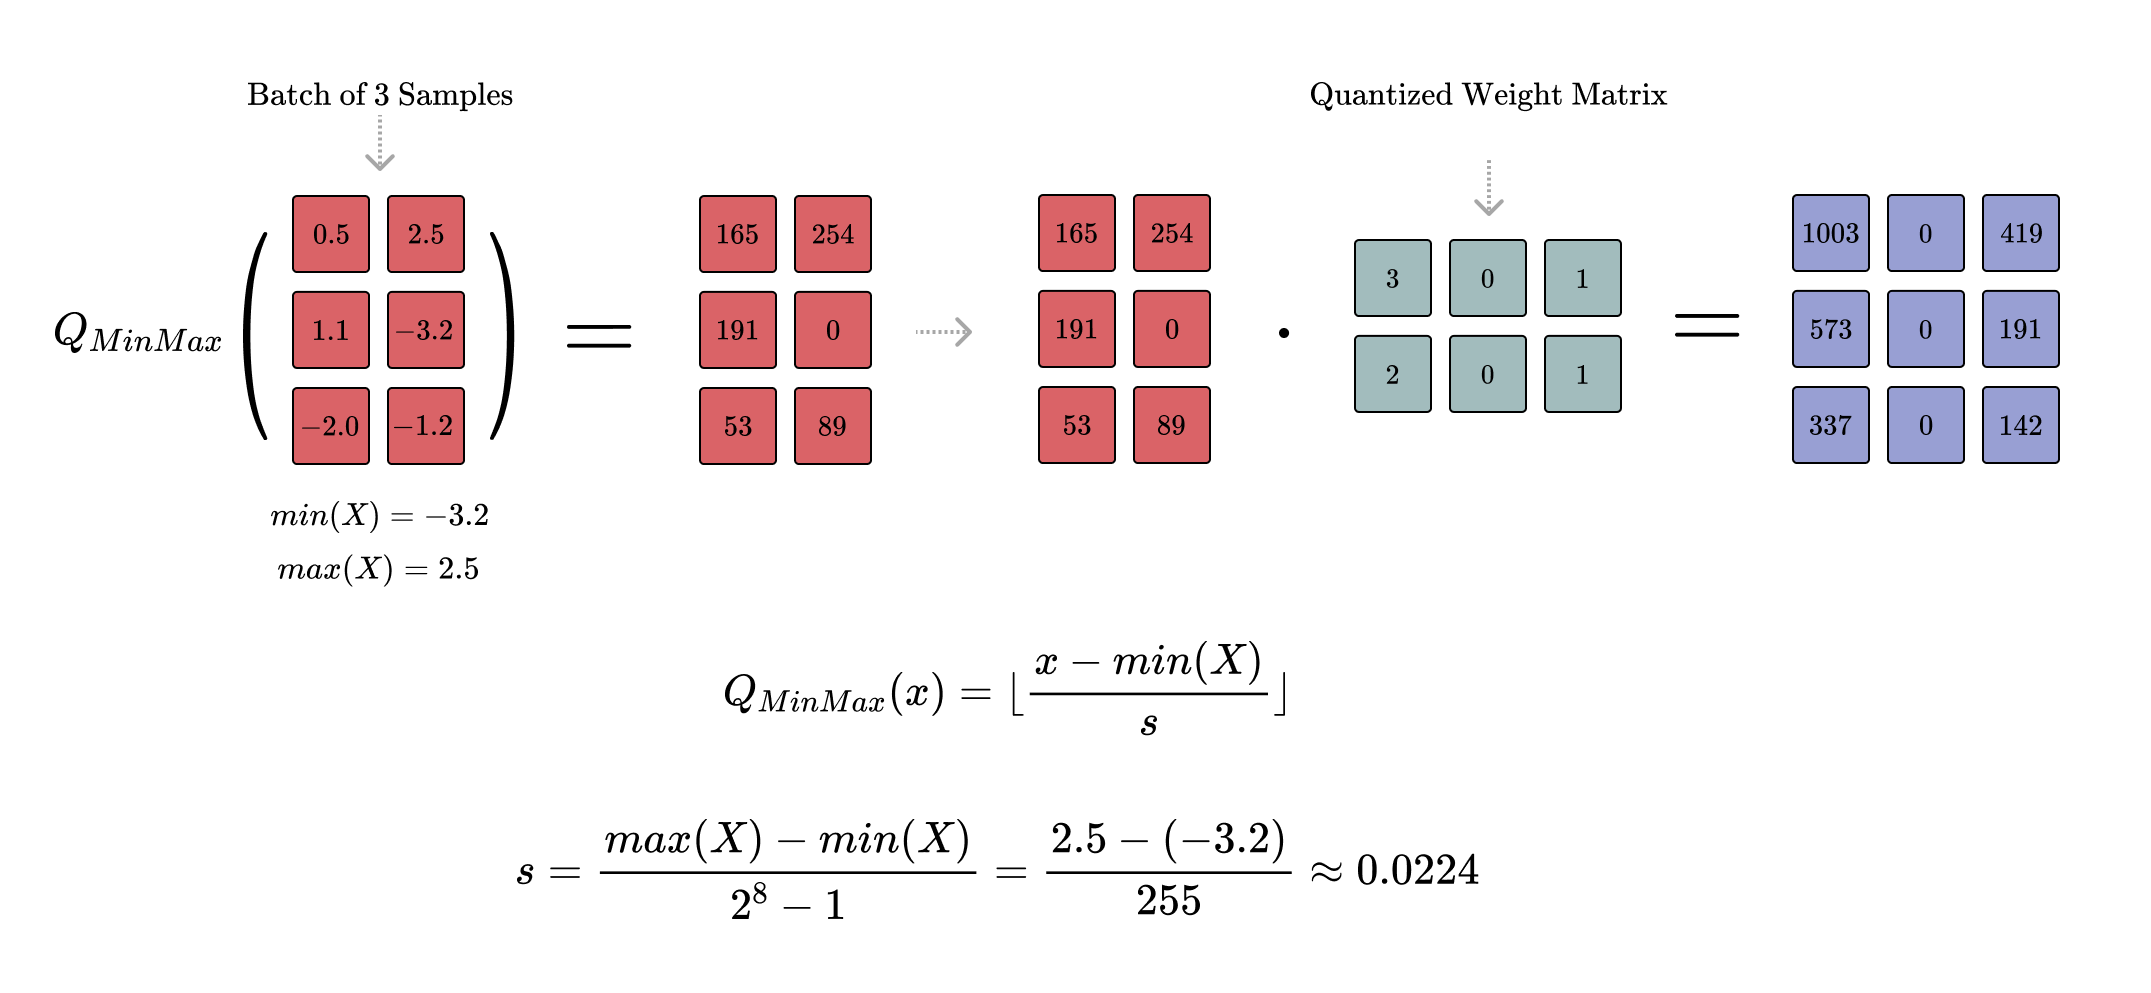
\includegraphics[width=15cm]{min_max_quantization.png}
  \caption{ An example illustrating min-max quantization of input data to 8 bits, followed by matrix multiplication with the quantized weight matrix from Figure \ref{fig:quantizing_example}.
  Input data has arbitrary values for demonstration purposes.}
  \label{fig:min_max_quantization}
\end{figure}

    \begin{itemize}
        \item In \textbf{static quantization}, quantization parameters are fixed before model inference, based on the data observed during training or calibration.
        This corresponds to Post-Training Quantization (PTQ), which directly quantizes the trained floating-point model \cite{jiang2021efficient}, 
        using various discretization approaches based on the range and distribution of the parameters being quantized, 
        as well as the level of granularity at which the quantization values are applied.
        
        \item In \textbf{dynamic quantization}, the quantization parameters are calculated dynamically during inference. 
        This typically applies to activations, as their range changes depending on the input data and, unlike that of the weights, 
        cannot be precomputed with static quantization \cite{kim2021ibert}.
        
        \item In \textbf{learned quantization}, quantization parameters are learned as part of the model training process.
        This corresponds to Quantization Aware Training (QAT) \cite{jacob2018quantization}, where quantization is integrated directly into training rather than applied afterwards.
        Since learned quantization is central to this work, a detailed review of QAT and its applications is provided in the Related Work chapter. 

    \end{itemize}

% ----------------------- third section

\section{Learned Quantization}
\label{sec:section3}
Now that the fundamentals of quantization have been covered, 
this section introduces key concepts commonly encountered in learned quantization,
including its challenges, trade-offs, and the popular techniques used to overcome them.

\subsection{Strategies and Applications}
\label{subsec:subsection1}
This

\subsection{Trade-offs and Challenges}
\label{subsec:subsection2}

%\subsection{Low-Precision Forward-Pass}
%\label{subsec:subsection1}
%In QAT, the operation performed during the forward-pass is often modified. Instead of propagating the full precision values, 
%the output of a layer is first quantized and then dequantized before being passed to the next layer \cite{jacob2018quantization}. 
%This simulates the effect of quantization during inference, helping the network adjust to the reduced precision parameters.
%\\
%\\
%The \textit{quantization} process can be generalized as follows:
%
%\[
%q(x) = \text{round}\left( \frac{x}{P} \right) - Z
%\]
%\\
%\noindent where \( q(x) \) is the quantized value, \( x \) is the full precision value of the parameter that is being quantized, \( P \) is a quantization parameter, such as a scaling factor, 
%and \( Z \) represents the zero point. This method is the most commonly used \textit{uniform quantization}, which can be either \textit{asymmetric} or \textit{symmetric}, 
%depending on the value of \( Z \), with  \( Z \) = 0 representing \textit{symmetric quantization}.
%\\
%\\
%For \textit{dequantization}, we apply:
%
%\[
%x_{\text{dequant}} = P \cdot ( q(x) + Z)
%\]
%\\
%\noindent Note that the dequantized value does not necessarily match the initial value. 
%For example, if \( x = 7.8 \) and \( P = 2 \), then quantization gives \( q(x) = 4 \), and dequantization results in \( x_{\text{dequant}} = 8 \). 
%This demonstrates how the \textit{quantization} and dequantization process approximates the original value \( x \)
%by rounding it to the nearest representable value based on the quantization parameter \( P \).

%\subsection{Full-Precision Back-Propagation}
%\label{subsec:subsection1}
%In QAT, although the forward-pass operates on quantized values, back-propagation typically uses full-precision values. 
%This is because the rounding operation in the forward-pass is non-differentiable, which makes it impossible to compute gradients directly \cite{polino2018modelcompression}.
%\\
%\\
%Consider the example of computing the gradient of the weight \( W_{I1,H1_1} \) in Figure~\ref{fig:mlp_diagram}:
%
%\[
%\frac{\partial L}{\partial W_{I1,H1_1}} = \frac{\partial L}{\partial \text{Output 1}} \cdot \frac{\partial \text{Output 1}}{\partial H1_1} \cdot \frac{\partial H1_1}{\partial W_{I1,H1_1}}
%\]
%\\
%\noindent If the output of \( H1_1 \) was quantized using a rounding operation, the gradient 
%\[
%\frac{\partial H1_1}{\partial W_{I1,H1_1}} 
%\]
%would be undefined due to the non-differentiability of rounding. This would break the gradient flow, making it impossible to update  \( W_{I1,H1_1} \)
%during back-propagation.
%\\
%\\
%To work around this, techniques such as the Straight-Through Estimator (STE) are commonly used \cite{bengio2013estimating} \cite{fan2021training} \cite{zhuang2018towards} \cite{krishnamoorthi2018quantizing}.
%The STE approximates the gradient by treating the rounding function as if it were differentiable during the back-propagation.
%This approach ensures that the model can simulate low-precision inference during the forward pass,
%while still benefiting from the accuracy of full-precision gradient updates during back-propagation.
%\\
%\\
%The Experimental Setup section will explain a slighly different version of the typical STE that was used in the current work.

THIS PART WILL GO TO THE NEXT SECTION:
\\
\\
An example approach is to define a regularization term that directly penalizes large differences between full-precision values 
and their quantized counterparts \cite{zhuang2018towards}. This can encourage the model to learn parameters that are easily quantizable without significant performance loss.
If the values that are being quantized are \( W \), then this regularization term could look like:

\[
\mathcal{L}_{\text{quant}} = \lambda \sum_{i} \| W_i - q(W_i) \|^2
\]

\noindent Where:
\begin{itemize}
    \item \( \lambda \) is a scalar that controls the importance of the quantization penalty.
    \item \( W_i \) represents the full-precision weight value before quantization at index \( i \).
    \item \( q(W_i) \) represents the quantized version of \( W_i \).
\end{itemize}

\noindent The current work uses multiple custom regularization terms that trigger the quantization process during training. 
These will be discussed in detail in the Experimental Setup section.

    \chapter{Learned Quantization\label{cha:chapter3}}
This chapter elaborates on the problem that this thesis tries to solve and explains the individual methods used for solving the problem. 


\section{Custom Quantization Layers}
\label{sec:section1}

\subsection{Data Quantization Layer}
\label{subsec:subsection1}

\subsection{Parameter Quantization Layer}
\label{subsec:subsection2}

\subsection{Quantized Dense Layer}
\label{subsec:subsection3}

\section{Custom Loss Functions}
\label{sec:section2}

\subsection{Penalty for Inverse Scale Factor Magnitude} \label{subsec
}

\subsection{Constraint on Bin Count for Quantization} \label{subsec
}

\subsection{Deviation between Quantized and Original Values} \label{subsec
}
    \chapter{Experiments\label{cha:chapter4}}
This chapter provides details about the experiments conducted within the context of this thesis. 


\section{Experimental Setup\label{sec:setup}}
All experiments are caried out on machine XYZ. 

\section{Hyperparamter Tuning\label{sec:datasets}}

\section{Dataset-Specific Results\label{sec:datasets}}



%\section{Results for Experiment A\label{sec:results1}}
%Figure~\ref{fig:aliceandbob} illustrates the situation between Alice and Bob. (sequence diagram from www.websequencediagrams.com)

%\begin{figure}[htb]
%  \centering
%  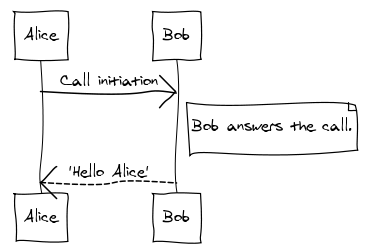
\includegraphics[width=9cm]{uml_seq_example.png}\\
%  \caption[Example figure]{Alice and Bob}
%  \label{fig:aliceandbob}
%\end{figure}

%\section{Results for Experiment B\label{sec:results2}}
%In Table~\ref{table:example} the statistics for...

%\begin{table}[H]
%  \begin{center}
%  \begin{tabular}{ | p {2.5cm}| p{3.6cm}| p{3.6cm}| p{3.3cm}| }
%  \hline
%  \textbf{Dateset} & \textbf{Minimum y} & \textbf{Maximum y} & \textbf{Average y} \\
%  \hline
%  DS 1 & -68.57 & 506.78 & 86.05 \\ \hline
%  DS 2 & -0.18 & 537.67 & 102.51 \\
%  \hline
%  \end{tabular}
%  \caption[Example table]{This table shows the statistics (minimum, maximum, and average) for the different datasets.}
%  \label{table:example}
%  \end{center}
%\end{table}


%\section{Discussion of Results\label{sec:resultDiscussion}}
%...

    \chapter{Related Work\label{cha:chapter5}}

A significant amount of scientific work has been done on QAT. 
This research can be categorized based on different characteristics, 
which are covered separately in the following paragraphs.

\noindent
\textbf{Model architecture.}\\
RNN - \cite{ott2016rnn}
CNN - \cite{rastegari2016xnor}

\noindent
\textbf{Quantization target parameters.}\\
weights and activations - \cite{krishnamoorthi2018quantizing}\\
weights and activations - \cite{hubara2016qnn}\\
weights - \cite{polino2018modelcompression}
weigths - \cite{ott2016rnn}
weights and inputs - \cite{rastegari2016xnor}


\noindent
\textbf{Granularity of quantization.}

\noindent
\textbf{Handling of differentiability.}

\noindent
\textbf{Quantization precision.}\\
binary weights - \cite{courbariaux2015binaryconnect}
binary weights and activations - \cite{hubara2016qnn}
ternary weights - \cite{ott2016rnn}

\noindent
\textbf{Integration with pruning \& other techniques.}\\
pruning and Huffman Codign - \cite{han2016deepcompression}\\
distillation - \cite{polino2018modelcompression}

\noindent
\textbf{Modifications to loss functions.}

    \chapter{Conclusions\label{cha:chapter6}}

This chapter summarizes the contriubtions of the thesis and provides an outlook into future work. 

% ---------------------------------------------------------------
\backmatter % no page numbering from here
    \addchap{List of Acronyms}

\begin{tabbing}
spacespacespace \= space \kill
ML	 \> 	Machine Learning	 \\
\end{tabbing}
\endinput

		
		% if you want to provide a glossary with explanations of important terms put it in here

    % \bibliographystyle{geralpha}
    % \bibliography{./bib/manual}
    \printbibliography  
    \addchap{Appendix}

\begin{appendix}

Add additional experimental results that do not need to be directly included in the thesis body. 

\end{appendix}

\endinput


\end{document}
